\documentclass[a4paper]{article}
\usepackage[left=3cm,right=3cm,top=2cm,bottom=2cm]{geometry} % page settings
\usepackage{enumerate}
\usepackage{hyperref}
\usepackage{graphicx}
\usepackage{amsfonts}
\usepackage{amsthm}
\usepackage{mathtools}
\usepackage{titlesec}
\usepackage{polski}
\usepackage{tikz}
\usepackage[utf8]{inputenc}
\DeclarePairedDelimiter\ceil{\lceil}{\rceil}
\DeclarePairedDelimiter\floor{\lfloor}{\rfloor}
\DeclarePairedDelimiter\set{\lbrace}{\rbrace}
\newcommand{\rpm}{\raisebox{.2ex}{$\scriptstyle\pm$}}


\def\checkmark{\tikz\fill[scale=0.3](0,.35) -- (.25,0) -- (1,.7) -- (.25,.15) -- cycle;} 

\titlespacing*{\subsection}
{0ex}{10ex}{3ex}

\title{Lista 6}
\author{Kamil Matuszewski}
\date{\today}

\begin{document}

\maketitle
\setlength{\parindent}{0.5ex}
\setlength{\parskip}{1.5ex}
\newcommand{\R}{\mathbb{R}}
\newcommand{\N}{\mathbb{N}}


\begin{center}
\begin{tabular}{|c *{7}{|c} |c|}\hline
1 & 2 & 3 & 4 & 5 & 6 & 7 & 8 & 9\\
\hline 
\checkmark & \checkmark & \checkmark &\checkmark &\checkmark &\checkmark &\checkmark &\checkmark &\checkmark \\
\hline
\end{tabular}\\
\end{center}

\subsection*{Zadanie 1}
Mamy
$$D_n = \begin{vmatrix}
1 & -1 & -1 & \dots & -1\\
1 & 1\\
1 & & 1\\
\vdots & & & \ddots\\
1 & & & & 1 
\end{vmatrix} $$
Pokaż, że $det(D_n)=n$.

\begin{proof}
Okej. Dla $n=1, n=2$ trywialne. Załóżmy, że dla $n-1$ jest ok, sprawdzę dla $n$. Aby to zrobić skorzystam z Laprasa.\\
Rozwińmy to względem ostatniego wiersza. Patrząc na kolejne wyznaczniki macierzy $M_{ni}$ zobaczymy, że mnożymy je przez zera we wszystkich miejscach poza pierwszym i ostatnim elementem. Dla ułatwienia, najpierw pomińmy element pierwszy - do niego wrócimy za chwilę. Co do ostatniego, jeśli skreślimy ostatni wiersz i ostatnią kolumnę, otrzymamy $D_{n-1}$. Z założenia indukcyjnego, jej wyznacznik to $n-1$.\\
Teraz, niech $C_n$ będzie macierzą $D_n$ bez pierwszej kolumny i ostatniego wiersza. Z Laprasa i z obserwacji powyżej, wyznacznik $D_n$ to $znak \cdot det(C_n) + n-1$, gdzie znak to $(-1)^{n+1}$.
$$C_n = \begin{vmatrix}
-1 & -1 & \dots & -1\\
1\\
& \ddots\\
& & 1 & 0\\
\end{vmatrix} $$
Z pomocą eliminacji gaussa możemy ją łatwo sprowadzić do postaci
$$C_n = \begin{vmatrix}
0 & \dots & 0 & -1\\
1\\
& \ddots\\
& & 1 & 0\\
\end{vmatrix} $$
Znów zróbmy Laprasa tym razem względem pierwszego wiersza. Wyznaczniki $M_{1i}$ będą mnożone przez 0 poza ostatnim elementem. Wyznacznik macierzy z usuniętą pierwszą i ostatnią kolumną to 1. Mnożymy to przez $-1$ i znak. Znak to $(-1)^{n-1+1}$. Czyli wyznacznik $C_n$ to $(-1)^{n+1}$.\\
Wracając do wyznacznika $D_n$, jak już wcześniej wspomniałem, wynosi on $(-1)^{n+1} \cdot det(C_n) + n-1 = (-1)^{n+1} \cdot (-1)^{n+1} + n-1 = (-1)^{2(n+1)} +n-1$. Można łatwo zauważyć, że pierwszy składnik tej sumy to 1, niezależnie od $n$. Stąd otrzymujemy, że $det(D_n)=1+n-1=n$
\end{proof}

\clearpage
UWAGA! ROZWIĄZANIE INNE (SZYBSZE):
\begin{proof}
Weźmy nasze $D_n$. Zauważmy, że jeśli dodamy do pierwszego wiersza wszystkie kolejne dostaniemy:

$$D_n = \begin{vmatrix}
n & 0 & 0 & \dots & 0\\
1 & 1\\
1 & & 1\\
\vdots & & & \ddots\\
1 & & & & 1 
\end{vmatrix} $$

Czyli macierz dolnoprzekątniową. Wyznacznik tej macierzy to iloczyn liczb na przekątnej: $$n\cdot 1\cdot 1\cdot \dots \cdot 1 = n$$


\end{proof}


\subsection*{Zadanie 2}
Pokaż, że jeśli $X$ ma rozkład $Poisson(\lambda)$ to zachodzi $E(X^n)=\lambda E[(X+1)^{n-1}]$. Za pomocą tego związku policz $E[X^3]$.

\begin{proof}
$$E(X^n)=\sum\limits_{x=0}^{\infty} x^n \frac{\lambda^x e^{-\lambda}}{x!} \stackrel{*}{=} \sum\limits_{x=1}^{\infty} x^n \frac{\lambda^{x} e^{-\lambda}}{x!} = \lambda \sum\limits_{x=1}^{\infty} x^{n-1} \frac{\lambda^{x-1} e^{-\lambda}}{(x-1)!} =\lambda \sum\limits_{x=0}^{\infty} (x+1)^{n-1} \frac{\lambda^{x} e^{-\lambda}}{x!}=\lambda E[(X+1)^{n-1}]$$
$*$ - Zauważmy, że dla $x=0$ wyraz to $0$.
\end{proof}

Policzenie $E[X^3]$ zostawiam czytelnikowi jako ćwiczenie. Tu trzeba skorzystać z jakichś prostych własności, które wykorzystywaliśmy i dowodziliśmy na poprzednich listach.

\subsection*{Zadanie 3}
Zmienna $X$ ma rozkład $Poissona$. Jak wygląda $E(X!)$?

$$E(X!)=\sum_{x=0}^\infty x! \frac{\lambda^x e^{-\lambda}}{x!} =\sum_{x=0}^\infty \lambda^x e^{-\lambda} =e^{-\lambda} \frac{1}{1-\lambda}$$

\subsection*{Zadanie 4}
Oblicz $$I=\int_{-\infty}^{\infty}\int_{-\infty}^{\infty} e^{-\frac{1}{2}(x^2+y^2)}\ dx\ dy$$

Przenieśmy się na współrzędne biegunowe.\\
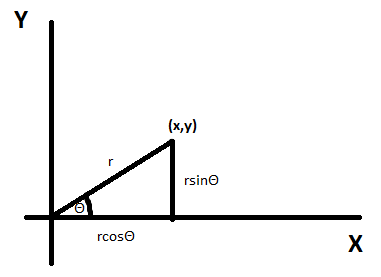
\includegraphics[scale=0.7]{zad4.png}\\
Widzimy, że w takim wypadku $x=r\cos{\theta}$ oraz $y=r\sin{\theta}$ Widzimy też, że $\theta \in [0^\circ,360^\circ]$ (lub inaczej $[0,2\pi]$), a $r \in [0,\infty)$. Teraz, wystarczy jakobian przekształcenia:
$$\begin{vmatrix}
\sin{\theta} & r\cos{\theta}\\
-\cos{\theta} & r\sin{\theta}
\end{vmatrix}=r $$
No i liczymy całeczkę:\\
$$\int_0^\infty \int_0^{2\pi} re^{-\frac{1}{2}r^2}\ d\theta\ dr = \int_0^\infty  re^{-\frac{1}{2}r^2} \int_0^{2\pi} 1 \ d\theta\ dr =  2\pi \cdot \left[-e^{-r^2/2}\right]_0^\infty = 2\pi$$


\subsection*{Zadanie 5}
Dane są niezależne zmienne losowe $X$, $Y$ o rozkładzie $U[0,1]$. Niech $x$, $y$ - wylosowane wartości zmiennych $X,Y$. Innymi słowy mamy odcinek $[0,1]$ i losujemy z niego $x$ i $y$, dzieląc go na trzy części. Musimy sprawdzić, jakie jest prawdopodobieństwo, że z tych trzech punktów utworzymy trójkąt.

Okej. To jest w sumie zadanie podobne do jakiegoś zadania z LO, tylko trochę bardziej skomplikowane (troszeczkę). Na początku, wiemy, że losowanie 2 punktów na prostej $[0,1]$ jest izomorficzne z losowaniem jednego punktu w przestrzeni $[0,1]x[0,1]$. To nam trochę ułatwi. Teraz, możemy zmniejszyć przestrzeń zdarzeń o połowę - pamiętając o tym i ostateczny wynik pomnożyć przez 2 - zakładając, że $x\leq y$. W naszej przestrzeni otrzymaliśmy trójkąt. Teraz, zastanówmy się jakie warunki muszą spełniać proste stworzone przez punkty, by dały się one złożyć w trójkąt. Trójkąt da się utworzyć, jeśli najdłuższy odcinek jest krótszy niż suma dwóch pozostałych. Nasz odcinek ma długość $1$, więc najdłuższy odcinek musi być mniejszy od $\frac{1}{2}$. Mamy zatem równania: $x<\frac{1}{2}$ - bo długość $[0,x]$ musi być mniejsza od $\frac{1}{2}$, jako, że jest to pierwszy punkt na prostej. Podobnie z $y$, tyko $y>\frac{1}{2}$, bo odcinek $[y,1]$ musi być krótszy niż $\frac{1}{2}$. Ostatni warunek, to odległość pomiędzy $x$ a $y$ musi być mniejsza od $\frac{1}{2}$, stąd $y-x<\frac{1}{2} \Rightarrow y<x+\frac{1}{2}$.\\
Rysujemy więc trzy proste. $x=\frac{1}{2}$, i zaznaczamy pole na lewo od niej ($x<\frac{1}{2}$), $y=\frac{1}{2}$ i zaznaczamy obszar na górze od niej ($y>\frac{1}{2}$), i prostą $y=\frac{1}{2}+x$, i zaznaczamy pole na dół od niej ($y<\frac{1}{2}+x$). Część wspólna tych obszarów wyznacza nam trójkąt. Całka po tym trójkącie da nam połowę prawdopodobieństwa z zadania (pamiętamy że podzieliliśmy przestrzeń zdarzeń na pół). Obrazek poniżej obrazuje (hehe) co zrobiliśmy:\\
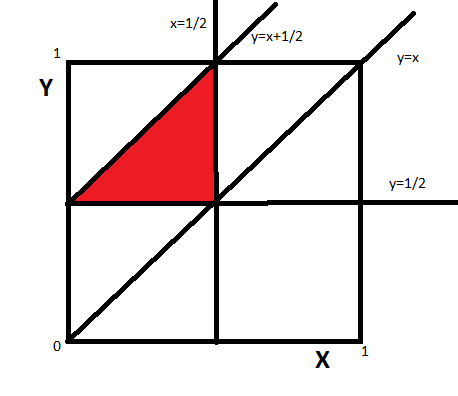
\includegraphics[scale=0.7]{zad5.png}\\
Czerwone pole to to co mamy policzyć.
Ustalmy sobie $x$. $0 \leq x \leq \frac{1}{2}$. Z prostej $y=x+\frac{1}{2}$, widać, że $\frac{1}{2} \leq y \leq x + \frac{1}{2}$. Mamy już wszystko. Obliczmy całkę:
$$\int_0^\frac{1}{2} \int_\frac{1}{2}^{x+\frac{1}{2}} 1\ dy\ dx = \frac{1}{8}$$
Pamiętamy, że wynik trzeba wymnożyć przez 2, więc wynik to $\frac{1}{4}$.

\subsection*{Zadanie 6}
Zadanie 5 dla gęstości $f(t)=2t$.

To jest zadanie 5, tylko inaczej liczymy ostatnią całkę. Zmienne są niezależne, $f(x)=2x$, $f(y)=2y$, $f(x,y)=4xy$.

Obliczmy całkę:
$$\int_0^\frac{1}{2} \int_\frac{1}{2}^{x+\frac{1}{2}} 4xy\ dy\ dx = \int_0^\frac{1}{2} 2x^2(x+1) dx =\left[ 2\left(\frac{x^4}{4} + \frac{x^3}{3}\right) \right]_0^\frac{1}{2}  = 2 \left( \frac{1}{64} + \frac{1}{24} \right) = \frac{1}{32} + \frac{1}{12} = \frac{11}{96}$$
Pamiętamy, że wynik trzeba wymnożyć przez 2, więc wynik to $\frac{11}{48}$.

\subsection*{Zadanie 7}
Mamy $f(x,y)=\frac{1}{\pi}$, dla $0<x^2+y^2<1$. Oblicz gęstości brzegowe $X$ i $Y$.

Po pierwsze zauważmy, że warunek $x^2+y^2>0$ gwarantuje nam jedynie, że $x$ i $y$ są niezerowe. Poza tym mamy $x^2+y^2=1$ i mamy policzyć pole pod nią. Widać, że jest to równanie okręgu o promieniu 1. Wiedząc to możemy bez problemu ustalić jakie mamy granice całkowania.\\
Dla ustalonego $x$, mamy $x^2+y^2<1 \Rightarrow y^2<1-x^2 \Rightarrow -\sqrt{1-x^2}<y<\sqrt{1-x^2}$. Dla ustalonego $y$ - analogicznie.

$$f(x)=\int_{-\sqrt{1-x^2}}^{\sqrt{1-x^2}} \frac{1}{\pi} dy = \frac{2\sqrt{1-x^2}}{\pi}$$
$$f(y)=\int_{-\sqrt{1-y^2}}^{\sqrt{1-y^2}} \frac{1}{\pi} dx = \frac{2\sqrt{1-y^2}}{\pi}$$

\subsection*{Zadanie 8}
Pokaż, że zmienne z zadania 7 są niezależne. Pokaż, że współczynnik korelacji wynosi 0.

To, że zmienne nie są niezależne widać od razu. Teraz, pokażę, że współczynnik korelacji wynosi 0.
\begin{proof}
$$p=\frac{\mu_{11}}{\sqrt{m_{20}m_{02}}} \ -\ wspołczynnik\ korelacji $$
Gdzie:
$$\mu_{11} = E[(X-EX)(Y-EY)]\ -\ moment\ centralny$$ 
$$m_{20}=E(X^2)\ -\ moment\ zwykły$$
$$m_{02}=E(Y^2)\ -\ moment\ zwykły$$

Okej. No to liczymy. Znów ustalamy sobie np. $x$. $x$ przebiega od $-1$ do $1$ (bo cały czas mówimy o okręgu o promieniu $1$)\\
$$E(X) = \int_{-1}^1 \int_{-\sqrt{1-x^2}}^{\sqrt{1-x^2}} \frac{x}{\pi}\ dy\ dx = \int_{-1}^1 \frac{2x \sqrt{1-x^2}}{\pi} dx = 0$$ 
$$E(Y) = \int_{-1}^1 \int_{-\sqrt{1-x^2}}^{\sqrt{1-x^2}} \frac{y}{\pi}\ dy\ dx = \int_{-1}^1 0 dx = 0$$
$$E(X^2) = \int_{-1}^1 \int_{-\sqrt{1-x^2}}^{\sqrt{1-x^2}} \frac{x^2}{\pi}\ dy\ dx = \int_{-1}^1 \frac{2x^2 \sqrt{1-x^2}}{\pi} dx = \frac{1}{4}$$ 
$$E(Y^2) = \int_{-1}^1 \int_{-\sqrt{1-x^2}}^{\sqrt{1-x^2}} \frac{y^2}{\pi}\ dy\ dx = \int_{-1}^1 \frac{2(1-x^2)^{\frac{3}{2}}}{3\pi} dx = \frac{1}{4}$$
$$E[(X-0)(Y-0)] = E(XY) = \int_{-1}^1 \int_{-\sqrt{1-x^2}}^{\sqrt{1-x^2}} \frac{xy}{\pi}\ dy\ dx = \int_{-1}^1 0 dx = 0$$
$$p=\frac{0}{\sqrt{\frac{1}{8}}}=0 $$

\end{proof}

\subsection*{Zadanie 9}
Niech $X_1=Y_1\cos{Y_2}$, $X_2=Y_1\sin{Y_2}$, $0<Y_1<1$, $0\leq Y_2 \leq 2\pi$. Znajdź gęstość $g(y_1,y_2)$ zmiennej $(Y_1,Y_2)$. Sprawdź czy $Y_1$ i $Y_2$ są niezależne.

To się robi jakoś tak, że oblicza się jakobian, mnoży się przez gęstość. WKa ułatwił zadanie bo mamy już podane granice całkowania, więc obliczenie zależności zmiennych robi się trywialne.

Coś w stylu:\\
Jakobian:
$$|J|=\begin{vmatrix}
\cos{Y_2} & Y_1\sin{Y_2}\\
\sin{Y_2} & -Y_1\cos{Y_2}
\end{vmatrix} = | -Y_1\cos^2{Y_2} - Y_1\sin^2{Y_2} | = |-Y_1| = Y_1$$
Gęstość:
$$f(y_1,y_2)=f(x_1,x_2)\cdot |J| = \frac{y_1}{\pi} $$
Gęstość $y_1$:
$$f(y_1)=\int_0^{2\pi} \frac{y_1}{pi}\ dy_2 = \left[ \frac{y_1 y_2}{\pi} \right]_{y_2=0}^{2\pi} = 2y_1 $$
Gęstość $y_2$:
$$f(y_2)=\int_0^1 \frac{y_1}{pi}\ dy_1 = \frac{1}{2pi} $$
Niezależność:
$$f(y_1,y_2)= \frac{y_1}{pi} = \frac{1}{2pi} \cdot 2y_1 = f(y_1) \cdot f(y_2)$$
Wychodzi, że są niezależne. Z dokładnością do poprawności metody (na 95\% poprawna).

\end{document}
